\section{Results}

%\begin{figure}
%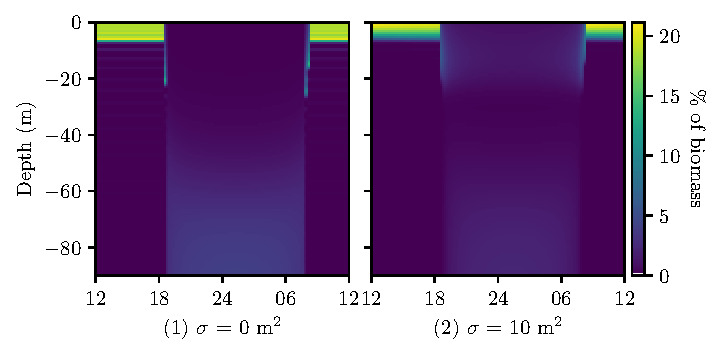
\includegraphics{plots/heatmapsday10_nonrandom.pdf}
%\caption{Vertical distribution of consumers \emph{(1)} and predators \emph{(2)} throughout the 1st of May, in hours from noon.}
%\end{figure}

\begin{figure}[H]
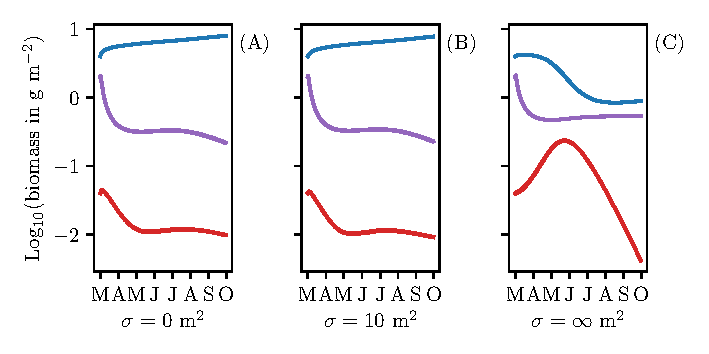
\includegraphics{plots/populations.pdf}
\caption{Total populations of consumers \emph{(blue)}, predators, \emph{(red)} and resources \emph{(purple)} from 1st of april to 1st of october. We vary the rationality, from total rationality \emph{(1)}, bounded rationality ($\sigma = 10...$), \emph{(2)} and fully irrational, $\sigma = \infty$, \emph{(3)}.}
\label{fig:long_term_populations}
\end{figure}
The difference in population dynamics between a system with no behavioral optimization, \Cref{fig:long_term_populations}(3), bounded rationality \Cref{fig:long_term_populations}(2) and full rationality \Cref{fig:long_term_populations}(1) is stark. The resources reach a stable level quickly in all three cases, but the populations of consumers and predators differ markedly. The difference in populations between the system with bounded rationality \Cref{fig:long_term_populations}(2) and the fully rational system appears to be negligible, \Cref{fig:long_term_populations}(1). The main driver seems to be the ability to retreat to a refuge, and not exactly how it happens.
%Large differences between irrational and the rational possibilities
\begin{figure}[H]
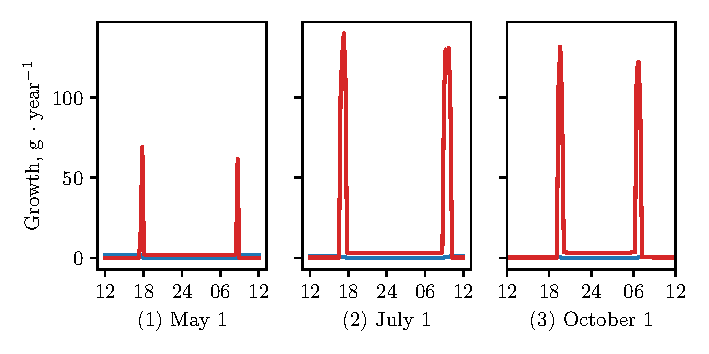
\includegraphics{plots/growth_short_rational.pdf}
\caption{Seasonal comparison of consumer \emph{(blue)} and predator, \emph{(red)} feeding patterns on 1st of May \emph{(1)}, 1st of July \emph{(2)} and 1st of October \emph{(3)}}
\label{fig:growth_short_rational}
\end{figure}
At all three points in time, consumers have a constant feeding level throughout the night \Cref{fig:growth_short_rational}. The main feeding time for predators is at dawn and dusk, with a slight peak during the day as well, \Cref{fig:growth_short_rational}. The length of predator feeding duration increases with the length of the night,  \Cref{fig:growth_short_rational}(2,3). Peak predator feeding activity decreases by a factor of 3/4 throughout the seasons, \Cref{fig:growth_short_rational}, reflecting lower maximal light levels.
\begin{figure}[H]
  \begin{centering}
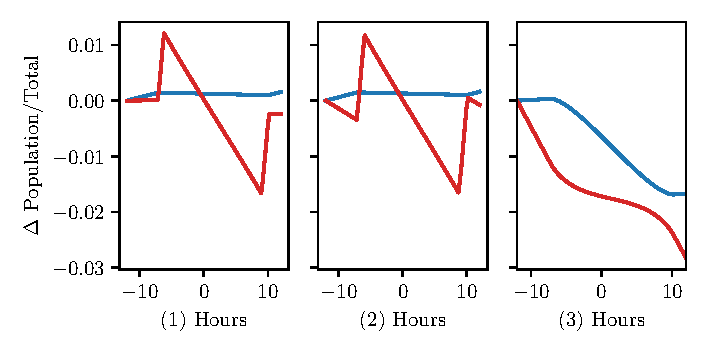
\includegraphics{plots/pop_dyn_comp_full_semi_none.pdf}
\end{centering}
\caption{Comparison of consumer \emph{(blue)} and predator, \emph{(red)} pr. capita growth patterns with complete rationality \emph{(1)}, bounded rationality \emph{(2)} and full irrationality \emph{(3)}}
\label{fig:pop_short_term}
\end{figure}
Looking at short-term population growth in the model with full rationality and bounded rationality, \Cref{fig:pop_short_term}(1,2), the change in consumer and predator populations throughout a day is on the order of $10^{-3}$. In contrast, the model with constant behavior has rather large fluctuations of populations through a single day \Cref{fig:pop_short_term}(3).
\begin{figure}[H]
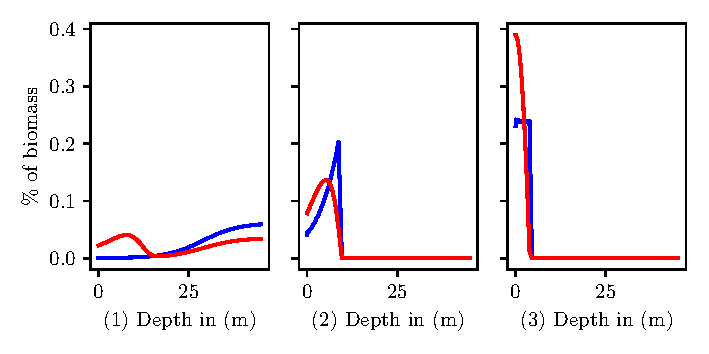
\includegraphics{plots/specific_dists_rational.pdf}
\caption{Daily distribution of consumers \emph{blue} and predators \emph{red} at noon \emph{(1)}, 18:45 \emph{(2)} and at midnight, \emph{(3)} with full rationality on the 1st of October}
\label{fig:specific_dists_rational}
\end{figure}
The driver of the daily production and growth cycles in the system with full rationality or bounded rationality is the vertical migration. At noon, \Cref{fig:specific_dists_rational}(1) the consumers form a deep scattering layer, where most of the predators are also present, excepting a few hanging out higher in the water column deterring upward consumer migration \Cref{fig:specific_dists_rational}(1)(15 m), corresponding to the modelling results of \citep{jerome}.

At dusk, \Cref{fig:specific_dists_rational}(2) the predators have a greater concentration near the surface, while the consumer "box" is begining to form, yet still with a continuous drop-off to the surface due to the risk from the light.
At midnight \Cref{fig:specific_dists_rational}(3) the consumers are concentrated near the surface, with a discontinuous drop to nothing. The predators follow the consumers, albeit with a continuous shape, both distributions being similar to the results of \citep{verticalmigration}.
\begin{figure}[H]
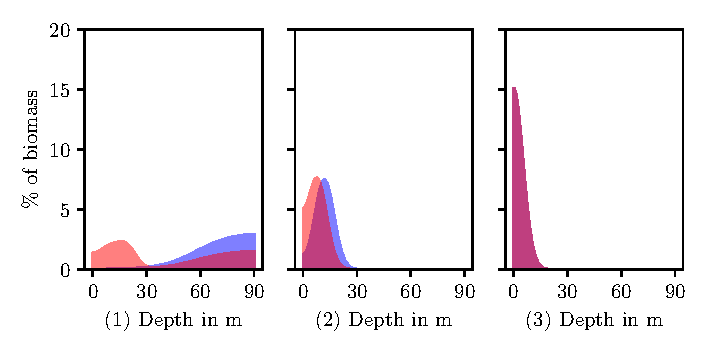
\includegraphics{plots/specific_dists_semi_rational.pdf}
\caption{Daily distribution of consumers \emph{blue} and predators \emph{red} at midnight \emph{(1)}, noon \emph{(2)} and at 18:45, \emph{(3)} with bounded rationality}
\label{fig:specific_dists_semi_rational}
\end{figure}
Examining snapshots of the migration in the ecosystem with bounded rationalty, \Cref{fig:specific_dists_irrational}, we see roughly the same picture as in \Cref{fig:specific_dists_rational}. The greatest difference is at midnight and dusk, \Cref{fig:specific_dists_irrational}(1,3), where the bounded rationality leads to a smooth shape for the distrbution of consumers. At noon, the distributions in the system with bounded rationality \Cref{fig:specific_dists_irrational}(2) and \Cref{fig:specific_dists_rational}(2) are almost entirely equal.
\begin{figure}[H]
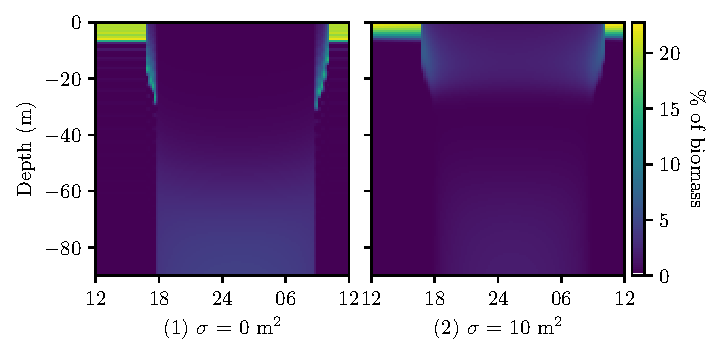
\includegraphics{plots/heatmapsday90_nonrandom.pdf}
\caption{Vertical distribution of consumers \emph{(1)} and predators \emph{(2)} throughout the 1st of July. The time is in hours from noon. }
\label{fig:heatmaps_90_nonrandom}
\end{figure}
To understand the migration in greater detail, we look at the complete migration picture.
The vertical migration of consumers, \Cref{fig:heatmaps_90_nonrandom}(1) is clear here in the middle of the summer.They are highly concentrated at the top of the water column during nighttime, and at day they scatter throughout the deep. The pattern of the predators is slightly different from the consumer pattern, \Cref{fig:heatmaps_90_nonrandom}. At nighttime there is still a non-zero concentration of predators in the upper layers of the water-column, there to catch any errant prey.
\begin{figure}[H]
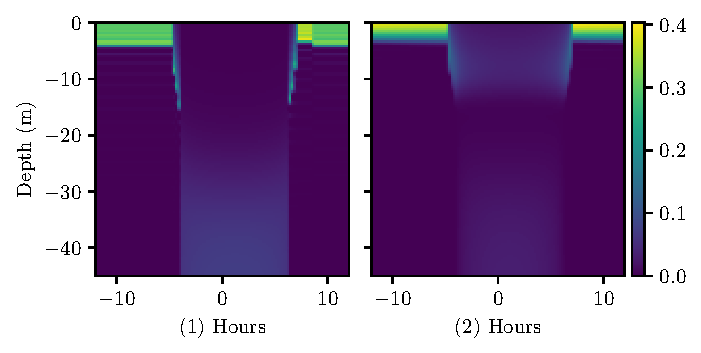
\includegraphics{plots/heatmapsday180_nonrandom.pdf}
\caption{Vertical distribution of consumers \emph{(1)} and predators \emph{(2)} throughout the 1st of October. The time is in hours from noon.}
\label{fig:heatmaps_180_nonrandom}
\end{figure}
Moving the hands on the clock forward to October, we again see a clearly defined vertical migration, \Cref{fig:heatmaps_180_nonrandom}. The migration differs from the previous migration, in that the descent and ascent are steeper, and the distributions are wider during the night.
